%Cabeçalho
\documentclass[12pt]{article}

%ABNT
\usepackage[UTF8]{inputenc}
\usepackage[lmargin = 3cm, tmargin = 3cm, rmargin = 2cm, bmargin = 2cm]{geometry}
\usepackage[onehalfspacing]{setspace}
\usepackage[T1]{fontenc}
\usepackage[brazil]{babel}

%Pacotes Essenciais
\usepackage{graphicx, xcolor, comment, enumerate, multirow, multicol, indentfirst}

%Pacotes de Matemática
\usepackage{amsmath, amsthm, amsfonts, amssymb, dsfont, blindtext}

%------------------------------------------------------------------
%Título
\title{Circuitos Elétricos II: Relatório Laboratório 1}
\author{Alexandre Abib e Rulian Dos Reis}
\date{\today}
%------------------------------------------------------------------
\begin{document}
	\maketitle
	\section{Introdução}
	Neste trabalho, o intuito foi entender o comportamento de circuitos RLC em série quando as entradas são funções degrau. Ao decorrer deste, analisamos quais possíveis saídas obtemos baseadas nos valores dos componentes dos circuitos e comparamos os resultados obtidos de forma prática, com o auxilio de um simulador, com os obtidos de forma teórica utilizando a teoria de circuitos e a Transformada de Laplace.
	\section{Análise do Circuito}
	Como dito anteriormente, o circuito analisado foi um circuito RLC deste formato:
	\begin{figure}[!h]
		\centering
		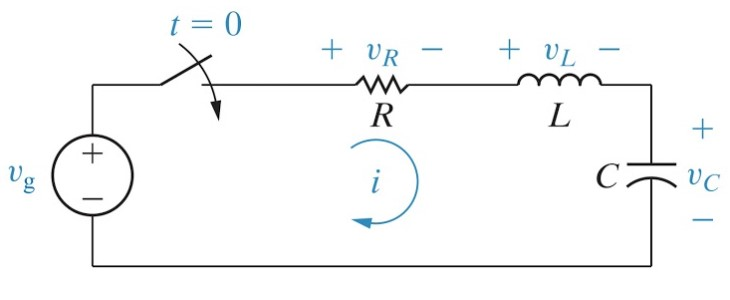
\includegraphics[width=12cm]{circuitoexemplo.jpg}
		\caption{Circuito geral}
	\end{figure}
	
	Com o circuito em mente, começaremos a alterar os valores dos componentes para obter as variações de saídas desejadas. As saídas podem assumir três formas: subamortecida, superamortecida e com amortecimento crítico. Cada uma dessas formas depende da relação entre duas variáveis que definiremos como "Alfa" e "Omega". Estas, por sua vez, são dadas por:
	\begin{equation}
		\alpha = \frac{R}{2L} , \omega_0 = \frac{1}{\sqrt{LC}}  
	\end{equation}


	\subsection{Resposta Subamortecida}
	A relação que define uma saída como subamortecida é 
	\begin{equation}
		\alpha^2 < \omega_0 ^2
	\end{equation}
	Nesse caso, 
	\begin{equation}
		i(t) = \frac{A}{L\beta}e^{(-\alpha t)}sen(\beta t)u(t)
	\end{equation}
	\begin{equation}
		vc(t) = [\frac{A}{LC(\alpha^2+\beta^2)} - \frac{A}{LC(\beta \sqrt{\beta^2 + \alpha^2)}}e^{-\alpha t}cos(\beta t + \arctan{\frac{\alpha}{\beta}})]u(t)
	\end{equation}
	Adotando os seguintes valores: 
	
	R = 280 ohms; 
	
	L = 0.1 Henrys;
	 
	C = 0.4 microFaradays; 
	
	V = 48 Volts. 
	
	O circuito se torna:
	\begin{figure}[!h]
		\centering
		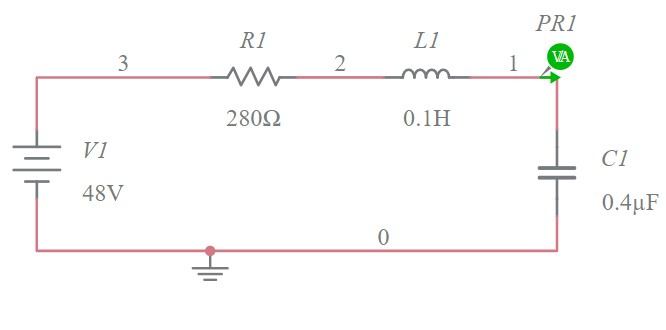
\includegraphics[width=12cm]{circuitoMultisimSub.jpg}
		\caption{Circuito no simulador Multisim}
	\end{figure}
	
	Comparando os gráficos obtidos no simulador e os obtidos analiticamente, temos:
	\newline
	\newline
	\begin{figure}[!h]
		\centering
		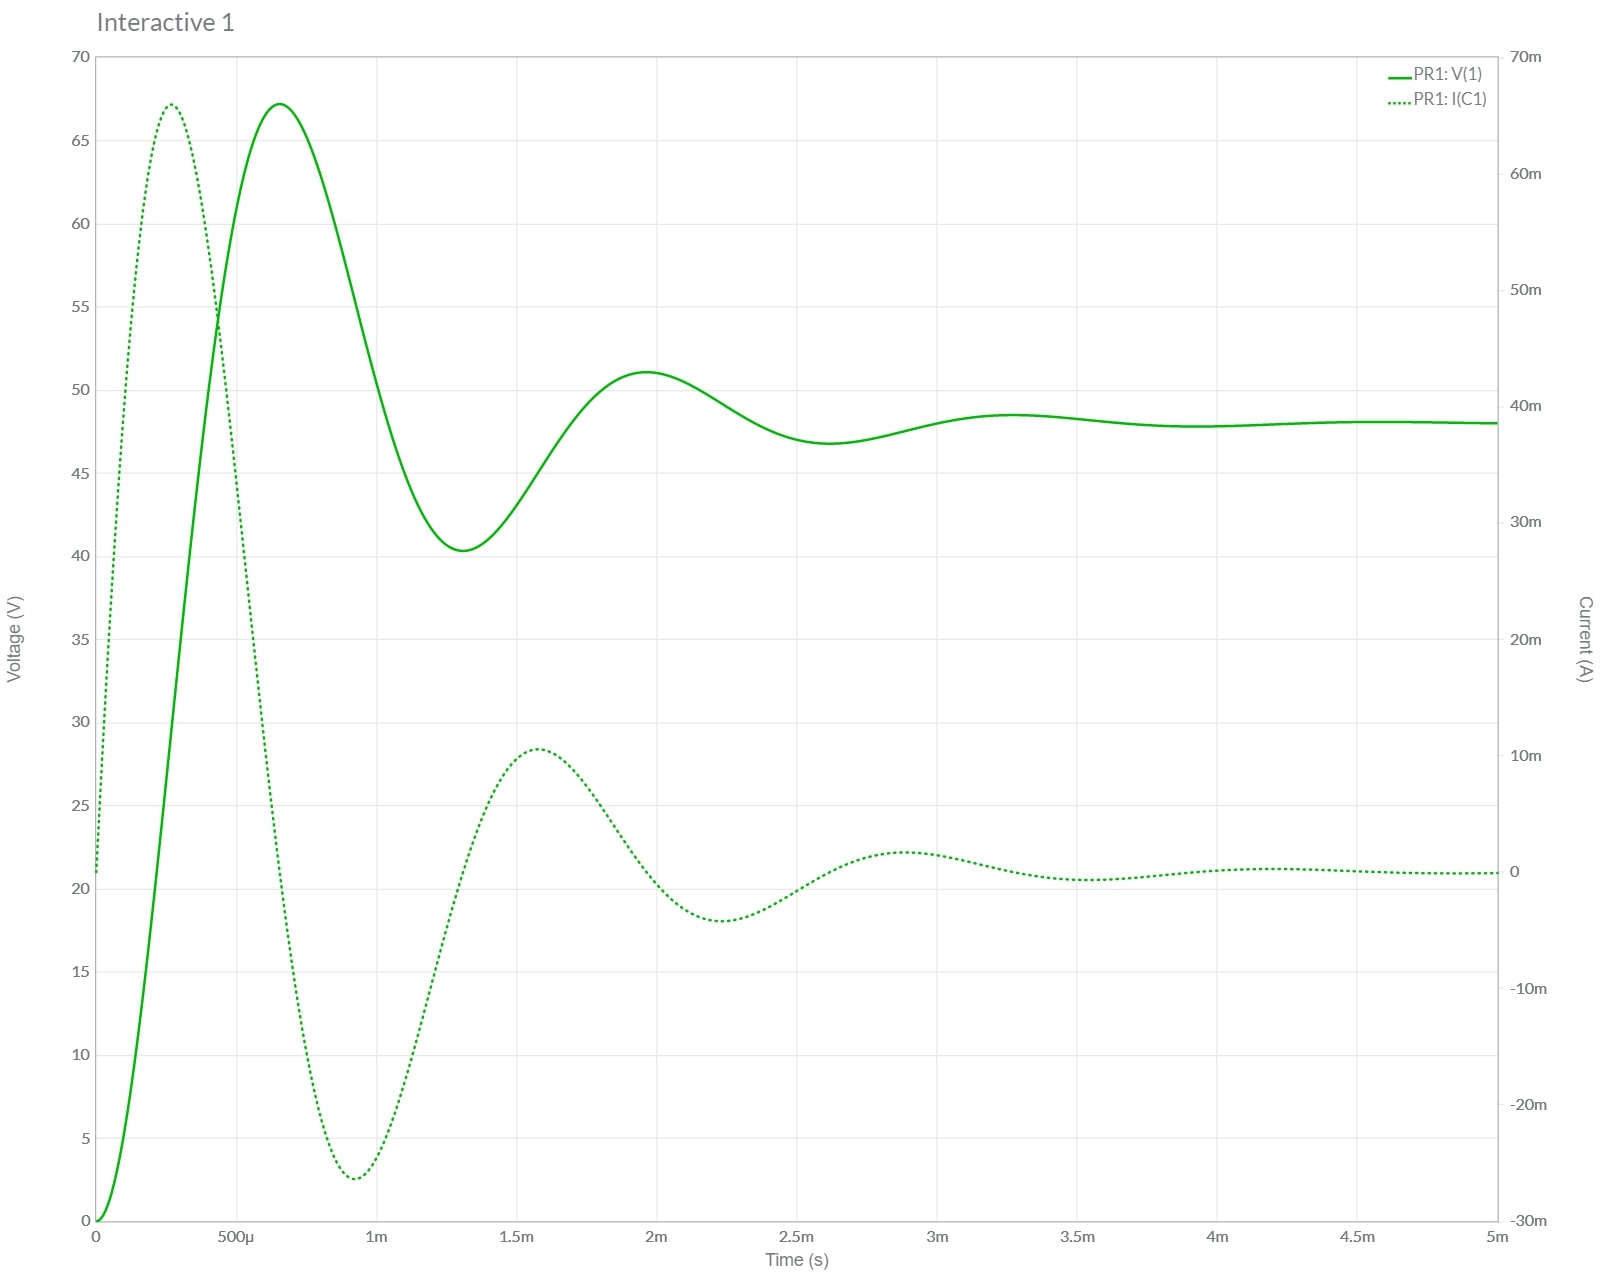
\includegraphics[width=12cm]{graficoMultisimSub.jpg}
		\caption{Gráfico do simulador Multisim}
	\end{figure}
	\begin{figure}[!h]
		\centering
		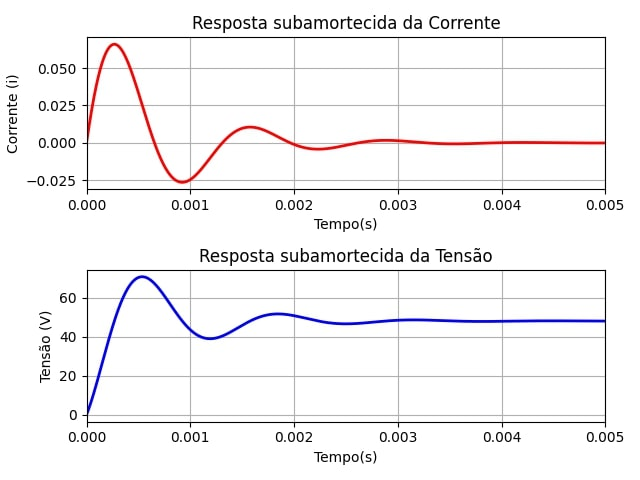
\includegraphics[width=12cm]{subPython.jpg}
		\caption{Gráfico gerado analiticamente pela biblioteca Matplotlib do Python}

	\end{figure}
	\pagebreak
	\newline
	\subsection{Resposta Superamortecida}
	A relação que define uma saída como superamortecida é

	\begin{equation}
		\alpha^2 > \omega_0 ^2
	\end{equation}
	Nessa caso,
	\begin{equation}
		i(t) = [\frac{A}{2L\beta}e^{-(\alpha - \beta)t} - \frac{A}{2L\beta}e^{-(\alpha+\beta)t}]u(t)
	\end{equation}
	\begin{equation}
		vc(t) = [\frac{A}{LC(\alpha^2 - \beta^2)} + \frac{A}{LC(2\beta^2 + 2\beta\alpha)}e^{-(\alpha+\beta)t} + \frac{A}{LC(2\beta^2 - 2\beta\alpha)}e^{-(\alpha - \beta)t}]u(t)
	\end{equation}
	Adotando os seguintes valores: 
	
	R = 25 ohms; 
	
	L = 0.25 Henrys;
	
	C = 2.5 miliFaradays;
	
	V = 150 Volts. 
	
	O circuito se torna:
	
	\begin{figure}[!h]
		\centering
		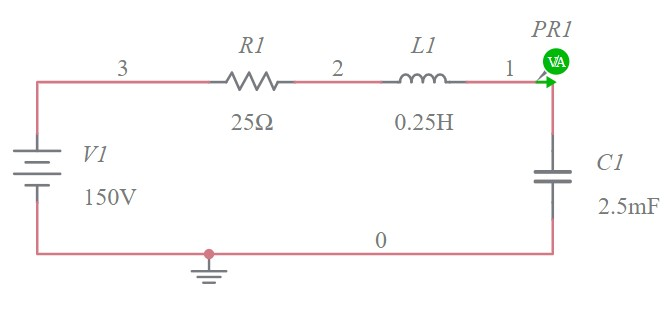
\includegraphics[width= 12cm]{circuitoMultisimSup.jpg}
		\caption{Circuito no simulador Multisim}
	\end{figure}
	
	Comparando os gráficos obtidos no simulador e os obtidos analiticamente, temos:
	
	\begin{figure}[!h]
		\centering
		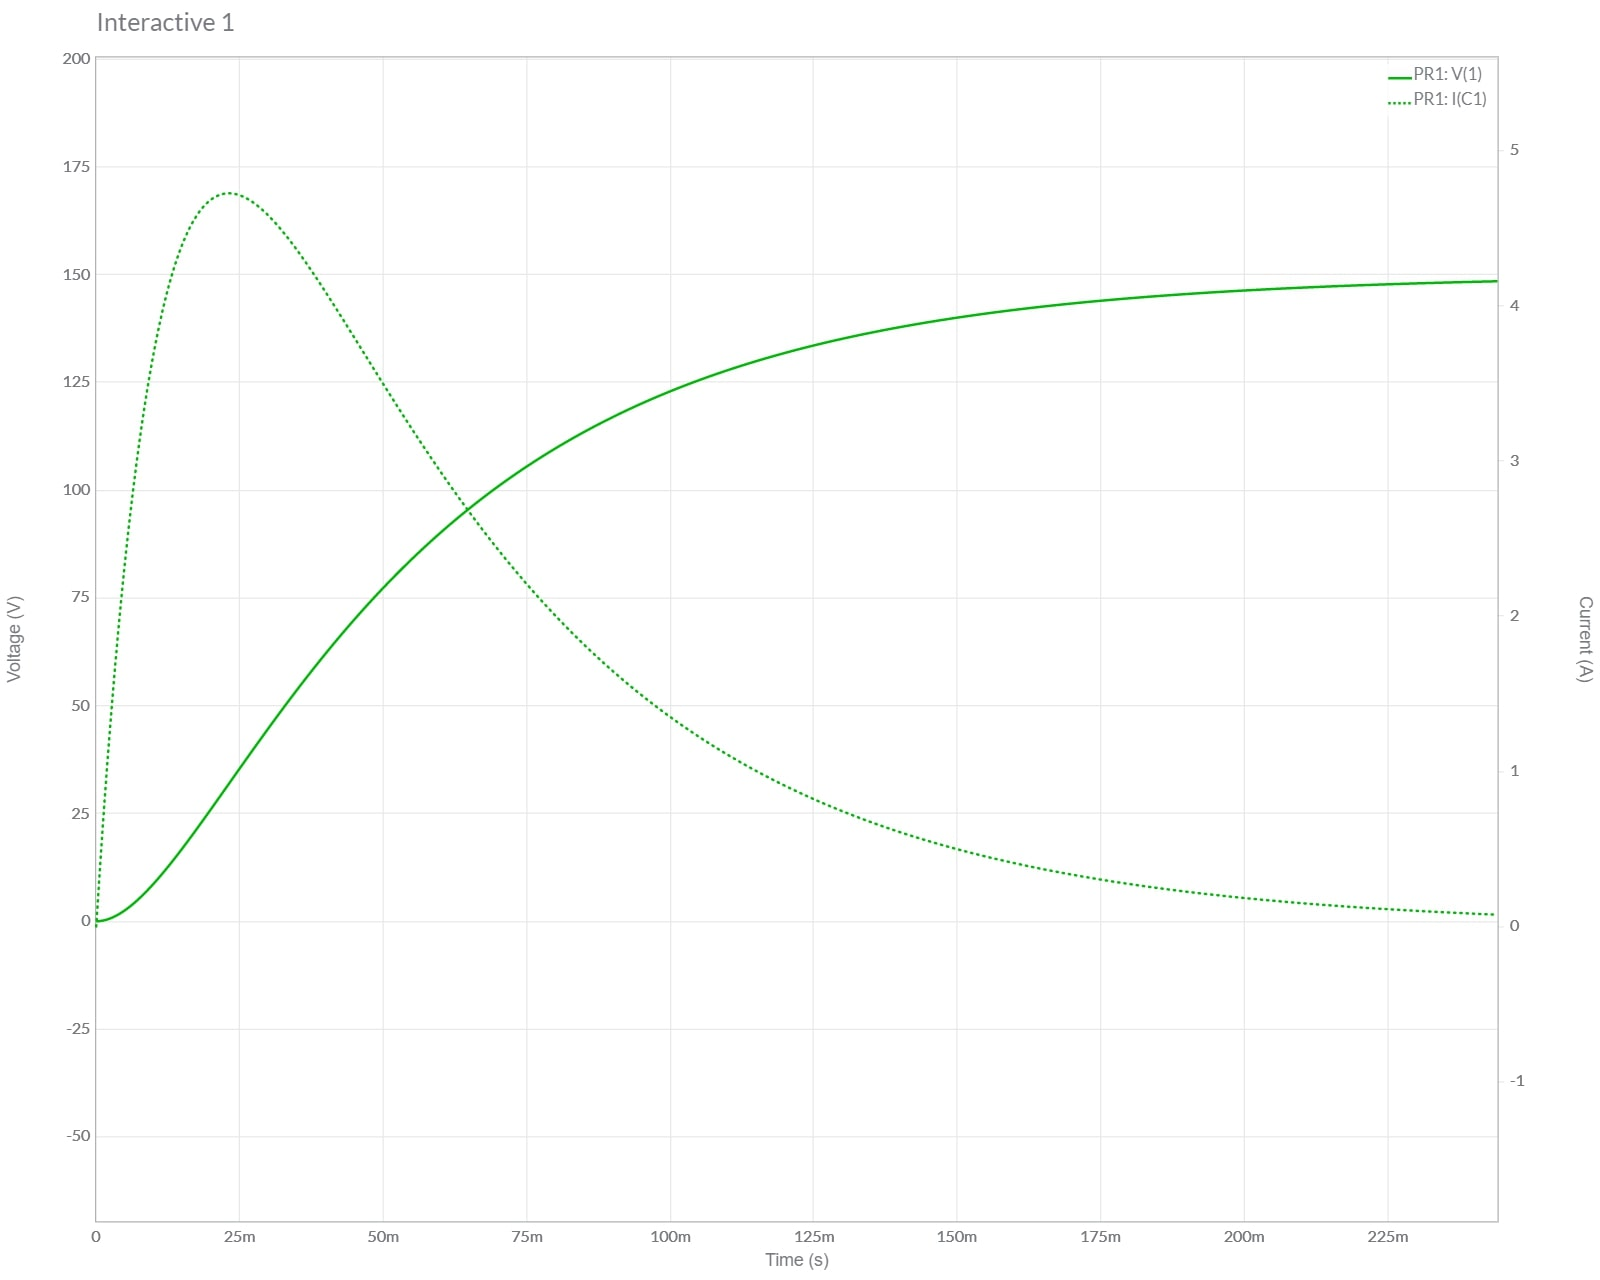
\includegraphics[width= 12cm]{graficoMultisimSup.jpg}
		\caption{Gráfico do simulador Multisim}
	\end{figure}
	\begin{figure}[!h]
		\centering
		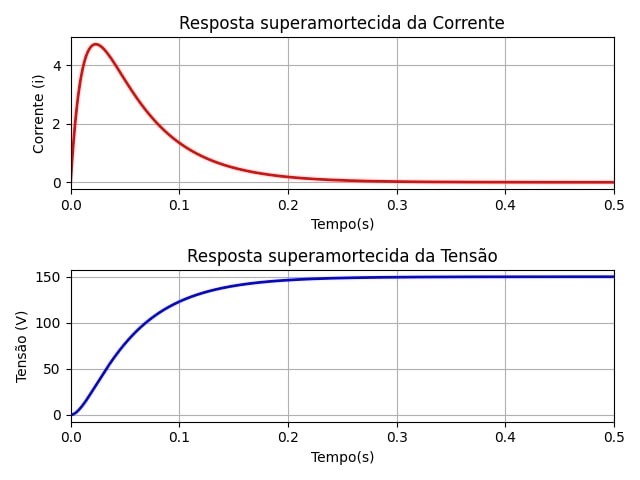
\includegraphics[width=12cm]{supPython.jpg}
		\caption{Gráfico gerado analiticamente pela biblioteca Matplotlib do Python}
	\end{figure}
	\pagebreak
	\vspace*{2cm}
	\subsection{Resposta Criticamente Amortecida}
	A relação que define uma saída como criticamente amortecida é 
	
	\begin{equation}
		\alpha^2 = \omega_0 ^2
	\end{equation}
	Nesse caso,
	\begin{equation}
		i(t) = \frac{A}{L}te^{-\alpha t}u(t)
	\end{equation}
	\begin{equation}
		vc(t) = [\frac{A}{LC\alpha^2 } - \frac{A}{LC\alpha}te^{-\alpha t} - \frac{A}{LC\alpha^2}e^{-\alpha t}]u(t)
	\end{equation}
	Adotando os seguintes valores: 

	R = 200 ohms; 
	
	L = 2 Henrys;
	
	C = 0.2 miliFaradays; 
	
	V = 50 Volts.
	
	O circuito se torna:
	
	\begin{figure}[!h]
		\centering
		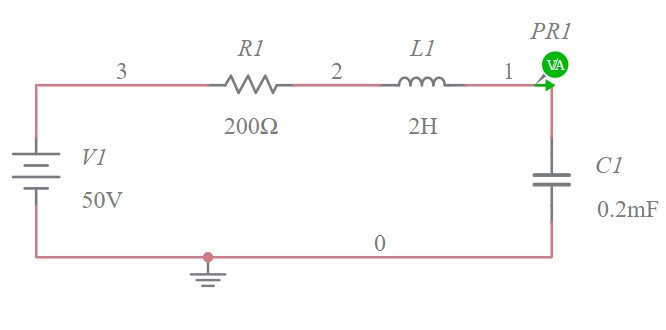
\includegraphics[width= 12cm]{circuitoMultisimCrit.jpg}
		\caption{Circuito no simulador Multisim}
	\end{figure}
	
	Comparando os gráficos obtidos no simulador e os obtidos analiticamente, temos:
	\begin{figure}[!h]
		\centering
		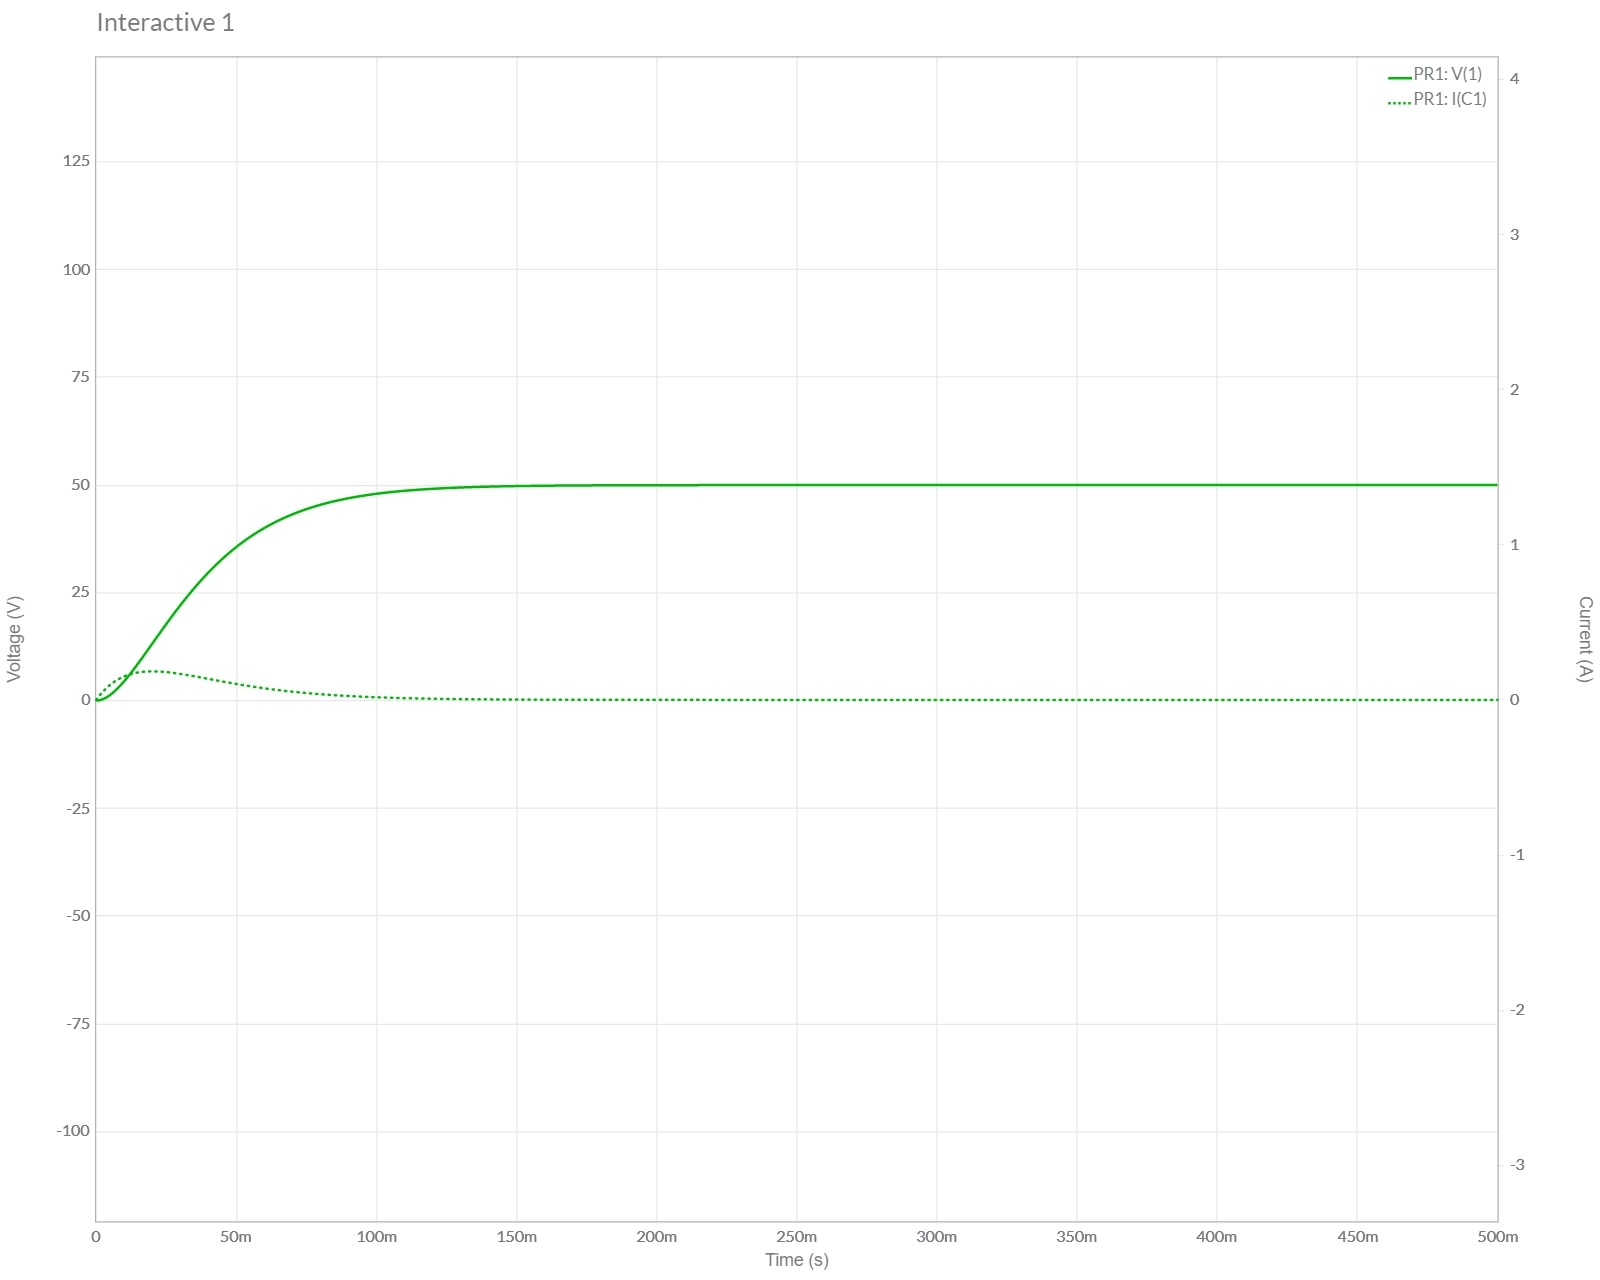
\includegraphics[width= 12cm]{graficoMultisimCrit.jpg}
		\caption{Gráfico do simulador Multisim}
	\end{figure}
		\begin{figure}[!h]
		\centering
		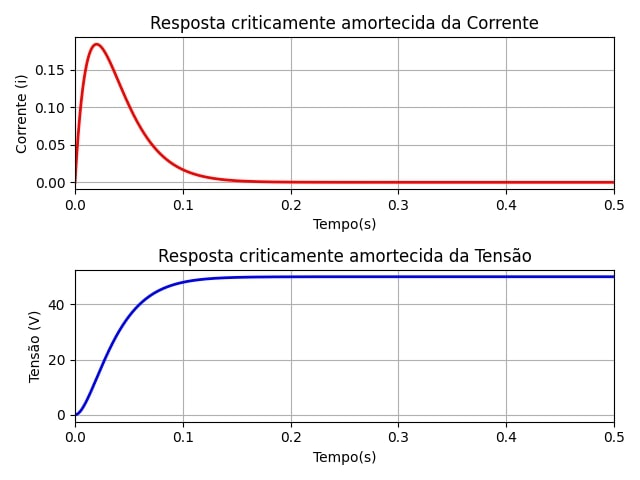
\includegraphics[width=12cm]{critPython.jpg}
		\caption{Gráfico gerado analiticamente pela biblioteca Matplotlib do Python}
	\end{figure}
	\pagebreak
	\vspace*{2cm}
	\section{Conclusão}
	
	
\end{document}